\documentclass[conference]{IEEEtran}
\IEEEoverridecommandlockouts
\usepackage[T1]{fontenc}
\usepackage{amsmath,amssymb,graphicx,booktabs,array,url,xcolor,tikz}
\usetikzlibrary{positioning,calc,arrows.meta}
\usepackage[hidelinks]{hyperref}
\graphicspath{{../figures/}}
% every experimental number in this paper is a macro generated from results/ by make_numbers.py
\input{numbers.tex}

\begin{document}

\title{How Far Can Simulation Take Vehicle-Based IRI Estimation? A Route-Disjoint Study on Profilometer-Referenced Car Data}

\author{
\IEEEauthorblockN{Nishkarsh Singhal}
\IEEEauthorblockA{\textit{Department of Electronics and Communication Engineering} \\
\textit{Faculty of Technology, University of Delhi}\\
New Delhi, India}
\and
\IEEEauthorblockN{Geetanjali Bhola}
\IEEEauthorblockA{\textit{Department of Computer Science and Engineering} \\
\textit{Faculty of Technology, University of Delhi}\\
New Delhi, India}
}

\maketitle

\begin{abstract}
Estimating the International Roughness Index (IRI) from the vibration of ordinary cars would make roughness monitoring cheap, and simulation is attractive because simulated roads come with exact labels.
Starting from a simulation-trained estimator of our own, we examine which conclusions survive validated labels and route-disjoint evaluation on public car data with profilometer IRI (LiRA-CD, \liraKm\,km, four routes).
Labels derived from game-engine road meshes with a curvature-adaptive correction were not IRI: on real profilometer profiles the correction lowers urban IRI by \legacyCorrUrbanMape\,\%.
On real cars, gradient boosting on vibration and speed features reaches a segment-level mean absolute error (MAE) of \liraGbmMae\,m/km (Spearman \liraGbmRho), indistinguishable from an MLP and better than a 1D-CNN (\liraCnnMae\,m/km) and a speed-only model (\liraSpeedMae\,m/km).
Speed is confounded with road class, and on a crowdsourced dataset without IRI it predicts the subjective quality labels better than vibration does.
Trained only on a randomised half-car and sensor simulator driven over measured profiles of other roads, the same estimator reaches \zsPsevenGbmMae\,m/km on real cars; a model trained on real data needs about 20\,km of profilometer-labelled road to match it, whereas training on the game-engine corpus does not transfer (\zsBngCorrGbmMae\,m/km).
In controlled simulations, learned speed corrections hold only for the road spectra seen in training, and no accurate estimator meets an unseen-vehicle criterion fixed in advance.
Simulation driven by measured profiles can thus replace scarce labels for the vehicle type tested, while claims of speed invariance and vehicle independence require controlled tests.
\end{abstract}

\begin{IEEEkeywords}
International Roughness Index, road roughness, vehicle vibration, connected vehicles, simulation-to-real transfer, evaluation protocol.
\end{IEEEkeywords}

\section{Introduction}
\label{sec:intro}
The International Roughness Index (IRI) is the standard summary of longitudinal road roughness~\cite{sayers1986tp45,astm_e1926}.
Measuring it requires a longitudinal profile, typically from an inertial laser profilometer, which is too expensive to survey minor roads frequently.
Ordinary vehicles that already carry accelerometers---smartphones, telematics units, connected cars---could close this gap if their vibration could be mapped to IRI~\cite{sattar2018review,sang2024iri,levenberg2021lira}.
Two obstacles recur: labelled data are scarce because each label requires a profilometer run, and the mapping from vibration to IRI depends on vehicle, mounting and driving speed~\cite{sayers1986tp46,thilak2021,mounting2026}.
Simulation is attractive for the first obstacle because the label of a simulated road is known exactly.

This paper started as a revision of our own earlier, unpublished study, which trained a CNN on vibration from the BeamNG.tech game engine, reported an MAE of 1.65\,m/km on a simulated test track, and claimed speed invariance and real-world validity from a crowdsourced dataset without IRI labels.
Re-examining that work revealed problems that are easy to make and hard to see in the final numbers: the labels were not IRI, the test track was also used for early stopping and calibration, test predictions above a threshold were discarded, and the crowdsourced labels were explained by driving speed.
Rather than polish that result, we asked which conclusions survive a protocol that excludes these failure modes, and we moved the main evaluation to public car data with profilometer labels.

We make four contributions.
(i) An IRI implementation that reproduces the P79 profilometer's reported IRI on public data ($r=$\,\iriValR{} over \iriValN{} segments), and evidence that the heuristic label correction used for game-engine roads lowers the IRI of real urban roads by \legacyCorrUrbanMape\,\% (Section~\ref{sec:res_labels}).
(ii) A quantification of how test-domain calibration and prediction filtering shaped our earlier results (Section~\ref{sec:res_protocol}).
(iii) A route-disjoint comparison of constant, speed-only, vibration-index, gradient-boosting, MLP and CNN estimators on \liraKm\,km of real car data with profilometer IRI, with segment-level uncertainty, and an analysis of speed as a confounder (Sections~\ref{sec:res_real}--\ref{sec:res_speed}).
(iv) Zero-shot and few-shot transfer from a randomised half-car and sensor simulator to real cars, and controlled tests of speed invariance, unseen vehicles and sensor robustness with criteria fixed in advance (Sections~\ref{sec:res_sim}--\ref{sec:res_controlled}).

In brief, simulation over measured profiles nearly matches real training (\zsPsevenGbmMae{} vs.\ \liraGbmMae\,m/km), but no accurate estimator meets our unseen-vehicle criterion, fixed in advance.
Code, protocol, configuration and all predictions are provided with the paper.

% Fig. 1 - study design. Real and simulated data share byte-identical preprocessing; all evaluation is route-disjoint.
\begin{figure*}[t]
\centering
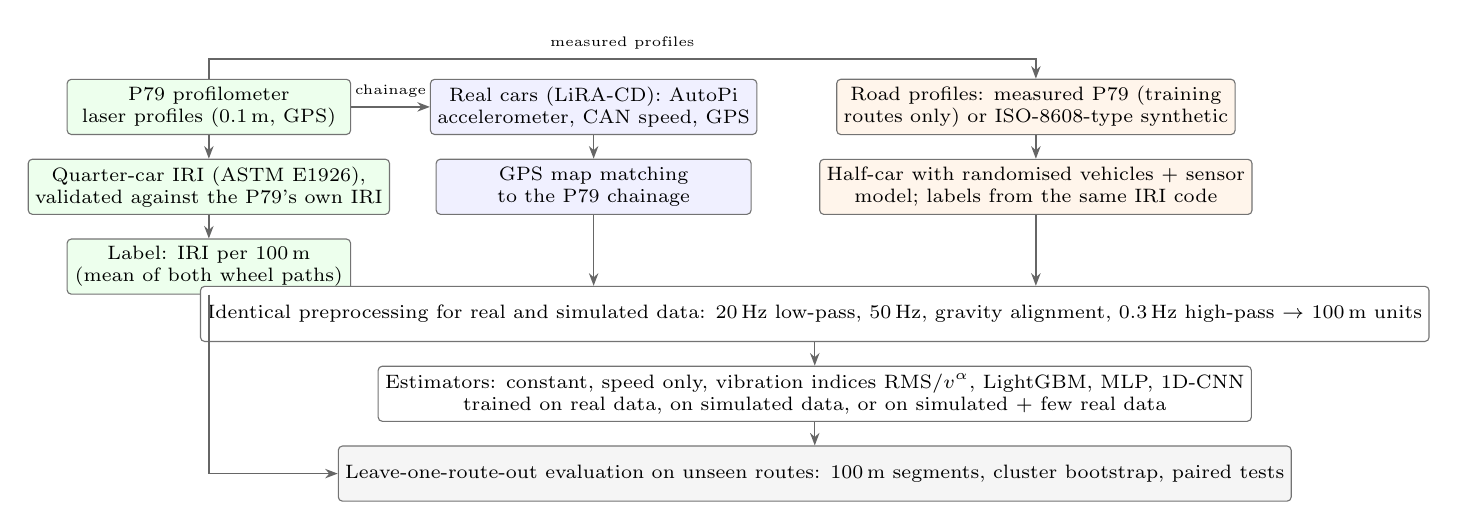
\begin{tikzpicture}[
  font=\scriptsize, node distance=3mm and 4mm,
  box/.style={draw=black!55, rounded corners=1.5pt, align=center, inner sep=2.5pt, minimum height=7mm, fill=white},
  real/.style={box, fill=blue!6}, sim/.style={box, fill=orange!8}, lab/.style={box, fill=green!7},
  arr/.style={-{Stealth[length=1.6mm]}, draw=black!60, line width=0.5pt}]
% reference labels (left column)
\node[lab, minimum width=36mm] (p79) {P79 profilometer\\laser profiles (0.1\,m, GPS)};
\node[lab, minimum width=36mm, below=of p79] (iri) {Quarter-car IRI (ASTM E1926),\\validated against the P79's own IRI};
\node[lab, minimum width=36mm, below=of iri] (lab100) {Label: IRI per 100\,m\\(mean of both wheel paths)};
% real cars (middle column)
\node[real, minimum width=40mm, right=10mm of p79] (car) {Real cars (LiRA-CD): AutoPi\\accelerometer, CAN speed, GPS};
\node[real, minimum width=40mm, below=of car] (mm) {GPS map matching\\to the P79 chainage};
% simulation (right column)
\node[sim, minimum width=44mm, right=10mm of car] (prof) {Road profiles: measured P79 (training\\routes only) or ISO-8608-type synthetic};
\node[sim, minimum width=44mm, below=of prof] (veh) {Half-car with randomised vehicles + sensor\\model; labels from the same IRI code};
% shared part
\node[box, minimum width=96mm, below=9mm of $(mm.south)!0.5!(veh.south)$] (pre) {Identical preprocessing for real and simulated data: 20\,Hz low-pass, 50\,Hz, gravity alignment, 0.3\,Hz high-pass $\rightarrow$ 100\,m units};
\node[box, minimum width=96mm, below=of pre] (models) {Estimators: constant, speed only, vibration indices RMS$/v^{\alpha}$, LightGBM, MLP, 1D-CNN\\trained on real data, on simulated data, or on simulated + few real data};
\node[box, minimum width=96mm, below=of models, fill=black!4] (eval) {Leave-one-route-out evaluation on unseen routes: 100\,m segments, cluster bootstrap, paired tests};
% arrows
\draw[arr] (p79) -- (iri);
\draw[arr] (iri) -- (lab100);
\draw[arr] (car) -- (mm);
\draw[arr] (prof) -- (veh);
\draw[arr] (p79.east) -- (car.west) node[midway, above, font=\tiny] {chainage};
\draw[arr] (p79.north) -- ++(0,2.5mm) -| (prof.north) node[pos=0.25, above, font=\tiny] {measured profiles};
\draw[arr] (mm.south) -- (mm.south |- pre.north);
\draw[arr] (veh.south) -- (veh.south |- pre.north);
\draw[arr] (pre) -- (models);
\draw[arr] (models) -- (eval);
\draw[arr] (lab100.south) |- (eval.west);
\end{tikzpicture}
\caption{Study design. Labels are recomputed from the P79 profilometer's laser profiles with an IRI implementation validated against the profilometer's own output; simulated units are labelled with the same code. Real and simulated vibration go through identical preprocessing, and every estimator is evaluated on routes it never saw.}
\label{fig:pipeline}
\end{figure*}

\section{Related Work}
\label{sec:related}

\textbf{Response-type roughness measurement.}
IRI is defined on the longitudinal profile through a reference quarter-car (the ``Golden Car'') driven at 80\,km/h~\cite{sayers1986tp45,sayers1995iri,astm_e1926}.
Measuring the response of an ordinary vehicle instead of the profile is a long-standing, cheaper alternative; such response-type systems are not self-calibrating and must be correlated with a reference profiler~\cite{sayers1986tp46}.
Model-based approaches estimate roughness from the responses of a specific vehicle, either with fixed vehicle models or with a vehicle model identified from drive tests and frequency-domain analysis~\cite{gonzalez2008accel,zhao2017freq}; Bridgelall's road impact factor normalises vertical-acceleration energy for connected vehicles~\cite{bridgelall2014rif}.

\textbf{Smartphones and connected vehicles.}
Crowdsourced road sensing started with event detection~\cite{eriksson2008pothole,mohan2008nericell}; a review summarises the many smartphone studies since~\cite{sattar2018review}.
Studies comparing smartphone estimates with reference roughness measurements report agreement that depends on speed, vehicle and phone~\cite{thilak2021}, on mounting~\cite{mounting2026}, and on the number of repeated runs~\cite{opara2022roughness}; see also~\cite{hanson2014iri}.
A data-driven model accounting for speed, vehicle type and mounting was trained on smartphone data from real vehicles~\cite{sang2024iri}, and semi-supervised learning has been used to exploit unlabelled responses of public or crowdsourced vehicles~\cite{zhang2026semisup,trc2021crowd}.
The LiRA project collected CAN-bus and accelerometer data from a fleet of production cars~\cite{levenberg2021lira}, released together with P79 profilometer surveys of the same lanes as LiRA-CD~\cite{skar2023lira}, the real-data backbone of this study; members of the project proposed a machine-learning pipeline that predicts roughness from car vertical acceleration and speed~\cite{bajic2021ml}.
An evaluation framework for smartphone roughness systems has been proposed in~\cite{evalframework2023}.

\textbf{Learning from simulated vehicle responses.}
Neural networks trained on simulated vehicle responses have been used to reconstruct road profiles and classify roughness~\cite{ngwangwa2010ann}, to classify roughness grades of white-noise road models from quarter-car simulations~\cite{rcnn2023sim}, and to build speed-adaptive roughness classifiers from quarter-car simulations and real-vehicle tests~\cite{speedadaptive2025}; a CNN was proposed for vehicle-calibration-free roughness assessment~\cite{jeong2020cnn}.
Game engines such as BeamNG.tech provide soft-body vehicles and are used in software-testing research~\cite{gambi2019beamng,beamng}, but the elevation of their authored road meshes is not a measured profile, so IRI labels derived from them need validation (Section~\ref{sec:res_labels}).
Domain randomisation is a standard device for simulation-to-real transfer~\cite{tobin2017dr}.
Compared with this work, we (i) validate the label computation against a profilometer, (ii) evaluate route-disjointly on public profilometer-referenced data from production cars, and (iii) separate roughness information from speed, which is confounded with road type in naturalistic driving.

\section{Research Questions and Hypotheses}
\label{sec:rq}
The study addresses five questions. The evaluation protocol, including splits, metrics and the two claim criteria below, was written down before any model was evaluated on a test route; it is part of the released material but was not registered with a third party.
\begin{itemize}
\item[\textbf{RQ1}] \emph{Label validity.} Does the IRI computation reproduce a reference profilometer, and does the curvature-adaptive ``mesh correction'' used to derive labels from game-engine road meshes preserve IRI?
\item[\textbf{RQ2}] \emph{Evaluation validity.} How much of a previously reported simulation result survives route-disjoint evaluation without calibration on, or filtering of, the test data?
\item[\textbf{RQ3}] \emph{Speed.} How much of the apparent skill is explained by driving speed rather than by vibration?
\item[\textbf{RQ4}] \emph{Real-car accuracy.} On unseen routes with profilometer IRI, how do constant, speed-only, vibration-index, gradient-boosting, MLP and CNN estimators compare?
\item[\textbf{RQ5}] \emph{Value of simulation.} Do estimators trained only on simulated vehicle responses transfer to real cars, and how much real labelled data does simulation replace?
\end{itemize}
RQ1--RQ3 test hypotheses formed in an earlier audit of our pipeline, before any experiment reported here: (H1) the mesh correction does not preserve IRI; (H2) the earlier result depends on calibration on, and filtering of, test data; (H3) driving speed explains a large part of the apparent skill.
RQ4 and RQ5 were asked without a directional hypothesis.
Two properties are tested in a controlled simulator with criteria fixed in advance: an estimator is called \emph{speed-invariant on [40,100]\,km/h} only if its mean prediction changes by less than $\pm$10\,\% between 40 and 100\,km/h on the same road (95\,\% CI inside the band), and it \emph{generalises to unseen vehicles} only if its MAE on unseen vehicle parameter sets is at most 10\,\% higher than on seen ones (upper CI bound).

\section{Data and Simulation}
\label{sec:data}
Table~\ref{tab:datasets} summarises the data sources and their role in the study.

\textbf{LiRA-CD (real cars, primary evidence).}
LiRA-CD~\cite{skar2023lira,lira_data} contains GreenMobility Renault Zoe car-sharing cars instrumented with an AutoPi telematics unit (three-axis accelerometer, GPS) connected to the CAN bus, and surveys of the same lanes by the Danish Road Directorate's P79 profilometer.
We use the four routes with car data: two urban roads in Copenhagen (CPH1, part of the O2 ring road, and CPH6) and two motorways (M3, M13), each in both directions.
The P79 files provide the wheel-path laser elevations at 0.1\,m with GPS and the profilometer's IRI per 10\,m.
In the \liraSensorPasses{} car passes with accelerometer data, the accelerometer is logged at a nominal \liraRateLow\,Hz (\liraRateLowShare\,\% of passes) or \liraRateHigh\,Hz with gaps (effective mean rates \liraRateMeanMin--\liraRateMeanMax\,Hz), quantised to 0.01\,g in \liraLsbShare\,\% of passes (otherwise \liraLsbMin\,g), and mounted with a median tilt of \liraTiltMedian$^\circ$ (95th percentile \liraTiltPninetyfive$^\circ$, one trip \liraTiltMax$^\circ$; angle between the static acceleration and the device's $z$ axis); speed comes from the CAN bus at \liraCanHz\,Hz and position from GPS at \liraGpsHzMin--\liraGpsHzMax\,Hz.
\liraSkipped{} passes lack accelerometer or speed data (\liraGpsOnly{} contain GPS only) and were skipped, and \liraNoUnits{} of the remaining \liraAllSignals{} passes yield no valid unit.
After map matching (Section~\ref{sec:method}), the dataset contains \liraUnits{} segment-passes over \liraSegments{} distinct 100\,m segments (\liraKm{}\,km) from \liraPasses{} car passes recorded by at least \liraDevices{} telematics units.
Urban segments have mean IRI \liraIriUrban{}\,m/km and are driven at \liraSpeedUrban\,km/h on average; motorway segments have mean IRI \liraIriMotorway{}\,m/km and are driven at \liraSpeedMotorway\,km/h.

\textbf{Earlier BeamNG corpus (game-engine simulation).}
The corpus of the earlier study comprises \bngTrips{} manually driven trips (one driver) of \bngCars{} BeamNG.tech vehicles on \bngMaps{} maps (\bngKm{}\,km of evaluation segments).
Elevation was sampled by downward ray casts next to the wheels; IMU, position and elevation were polled by unsynchronised threads, which produced exact sample-and-hold duplicates in \bngImuDupMin--\bngImuDupMax\,\% of consecutive IMU rows per trip.
Labels were computed from the ray-cast profile after a ``curvature-adaptive mesh correction'' that low-passes the profile where the 10\,m-smoothed curvature exceeds a threshold.
We use this corpus to answer RQ1--RQ3, not as a source of IRI ground truth.

\textbf{Parametric vehicle simulator.}
A linear four-degree-of-freedom half-car (bounce, pitch, front and rear unsprung masses) is driven by a road profile under the front axle and the same profile delayed by the wheelbase under the rear axle, after a 250\,mm tyre-envelope moving average.
The system is discretised exactly under a first-order hold and solved in modal coordinates; the solution deviates by at most \simModalDev{} (relative) from a direct state-space recursion and by \simRkDev{} from a fine-step Runge--Kutta integration of the continuous system, and the 500 sampled vehicles have body modes at \simBodyHzLo--\simBodyHzHi\,Hz and wheel-hop modes at \simHopHzLo--\simHopHzHi\,Hz.
Vehicle parameters are drawn from ranges for passenger cars~\cite{gillespie1992} that contain the Golden-Car reference vehicle~\cite{sayers1986tp45} (sprung mass 1000--1800\,kg, wheelbase 2.4--3.0\,m, body frequency 1.0--1.6\,Hz, damping ratio 0.20--0.45; Table~S1).
Speed is drawn independently of roughness (base speed 20--110\,km/h with Ornstein--Uhlenbeck fluctuations and random braking events).
The sensor model applies, in this order, an optional phone-holder resonance, the device's anti-aliasing filter, a mounting rotation, irregular sampling with jitter, scale and bias errors, white noise, quantisation and sample loss.
A telematics-like configuration (55--62\,Hz, 0.01\,g) and a smartphone-like configuration (90--210\,Hz, 0.6\,mg, holder resonance) are mixed 50/50.
The telematics configuration was set from a preliminary inspection of the unlabelled LiRA-CD streams, which was less accurate than the statistics above (Section~S1); it was not changed afterwards, and no LiRA-CD label was used to set any simulator parameter.
Two profile sources are used: the measured P79 profiles and ISO-8608-type synthetic profiles~\cite{iso8608} with displacement PSD $\propto n^{-2}$, roughness varying in 200--1000\,m sections and random potholes.
On measured profiles the half-car is driven by the mean of the two wheel-path profiles (no roll excitation), and units are labelled with the mean of the two wheel-path IRIs, exactly as the real units; on synthetic profiles the label is the IRI of the single driven profile.
All labels are computed with the validated IRI code (Section~\ref{sec:method}).

\textbf{PVS.}
The Passive Vehicular Sensors dataset~\cite{menegazzo2020pvs,menegazzo2021pvs} contains nine trips (three routes, each driven with three vehicles and drivers) with annotated surface type (asphalt, cobblestone, dirt) and subjective quality (good, regular, bad), but no IRI.
We use it only as ordinal, crowdsourcing-like evidence.

\begin{table}[t]
\centering
\caption{Data used in this study.}
\label{tab:datasets}
\setlength{\tabcolsep}{3pt}
\footnotesize
\begin{tabular}{@{}>{\raggedright\arraybackslash}p{0.17\columnwidth}>{\raggedright\arraybackslash}p{0.5\columnwidth}>{\raggedright\arraybackslash}p{0.27\columnwidth}@{}}
\toprule
Dataset & Content & Label; role \\
\midrule
LiRA-CD & Renault Zoe cars, AutoPi + CAN; 4 routes, \liraKm\,km of 100\,m segments, \liraUnits{} segment-passes & P79 IRI; training and test \\
Parametric simulator & randomised half-cars and sensors on measured (P79) and synthetic profiles & IRI of profile; training, controlled tests \\
BeamNG corpus & \bngCars{} game vehicles, \bngMaps{} maps, \bngTrips{} trips, \bngKm\,km & ray-cast profile IRI; RQ1--RQ3 \\
PVS & 3 cars, dashboard IMUs; 3 routes, \pvsWindows{} windows of 100\,m & surface type, quality; RQ3 \\
\bottomrule
\end{tabular}
\end{table}

\section{Method}
\label{sec:method}

\textbf{IRI computation.}
We implement the quarter-car algorithm of~\cite{sayers1995iri,astm_e1926}: the profile slope over a 250\,mm base (equivalent to a 250\,mm moving average), the Golden-Car state equations discretised with the matrix exponential for $\Delta t = \Delta x/(80\,\mathrm{km/h})$, initialisation with the average slope of the first 11\,m, and the rectified suspension-velocity slope accumulated along the profile.
The model is run once over a whole profile; the IRI of any window is the mean rectified slope inside it, which gives exact labels for overlapping windows and avoids per-window initialisation artefacts.
Two solvers (a reference loop and a linear-filter implementation) agree to \iriSolverDev\,m/km, a sinusoidal profile reproduces the analytical Golden-Car gain to a relative error of \iriSineDev, and a constant grade gives an IRI of \iriRampIri\,m/km.
Labels are the mean of the left and right wheel-path IRI per 100\,m.

\textbf{Shared preprocessing.}
Real and simulated accelerometer streams go through the same code: linear interpolation of the irregular samples to 200\,Hz, zero-phase 20\,Hz low-pass, decimation to 50\,Hz, projection on the pass-mean acceleration direction (which removes the static mounting tilt and gravity's orientation), conversion to m/s$^2$ and a zero-phase 0.3\,Hz high-pass that removes gravity, grade and slow attitude changes.
LiRA-CD GPS fixes are matched to the P79 track of the same route and direction (nearest vertex with a heading constraint, lateral distance $<$20\,m), split into runs of physically plausible progression (needed on the ring road) and interpolated in time.
A unit is a 100\,m segment of the P79 chainage traversed once and contiguously by one pass, with at least 90\,\% coverage and mean speed of at least 2\,m/s.

\textbf{Features and estimators.}
Every unit is described by speed (log mean speed, coefficient of variation) and vibration features of the dynamic vertical acceleration $a_z$: log RMS, 95th percentile and maximum of $|a_z|$, crest factor, kurtosis, band RMS in 0.5--2, 2--5, 5--10 and 10--15\,Hz, RMS after a 1\,Hz high-pass, and RMS at spatial wavelengths below 5\,m; the CNN receives $a_z$ resampled to 400 points over the 100\,m.
The estimators form a ladder of increasing flexibility:
M0, the training median;
M1, LightGBM~\cite{ke2017lightgbm} on the two speed features only;
M2, vibration indices $\log \mathrm{IRI} = a + b \log(\mathrm{RMS}\,a_z / v^{\alpha})$ with $\alpha = 0$ (M2a), $\alpha = 0.5$ (M2b, the exponent of body-acceleration RMS for a random road with displacement PSD $\propto n^{-2}$), $\alpha$ fitted by least squares on the training data (M2c), and $\alpha = 2$ (M2d, the exponent of the earlier study's kinetic normalisation, here applied after gravity removal);
M3, LightGBM on all features (and without the speed features);
M4, an MLP (64 and 32 units) on all features;
M5, the earlier study's dual-branch 1D-CNN (depthwise convolution, 48 and 64 filters, global average and max pooling, speed branch) re-implemented in PyTorch, with and without the speed branch;
M6, the member of \{M2c, M3, M4, M5\} with the lowest inner leave-one-route-out error on the training routes.
All learned estimators predict $\log(\mathrm{IRI})$.
Neural nets use a Huber loss, Adam, early stopping on a grouped 20\,\% hold-out of training segments, and five training seeds; on LiRA-CD and BeamNG we report the mean of the per-seed metrics, in the controlled simulation experiments the metrics of the seed-averaged prediction.
LightGBM selects one of six configurations, fixed in advance, by inner leave-one-route-out validation; without real training routes to validate on (zero- and few-shot), it uses the first configuration (7 leaves, at least 20 samples per leaf).
For RQ2 we also re-implement the earlier study's complete recipe (kinetic normalisation $a_z (v_{\mathrm{ref}}/v)^2$ of the gravity-including signal, asymmetric Huber loss, oversampling, two-dimensional inverse-frequency weights, isotonic calibration); on the earlier study's own tensors our re-implementation reaches MAE \legacyFidMae{}\,m/km and $R^2$ \legacyFidRtwo{} against the 1.650 and 0.521 reported in the earlier manuscript.

\textbf{Using simulation.}
\emph{Zero-shot}: an estimator is trained only on simulated units (synthetic profiles, measured P79 profiles of the three training routes, or both) and applied to the held-out real route; the held-out route's profile is never simulated for training.
\emph{Few-shot}: $k \in \{1,2,5,10,20\}$\,km of real labelled road (contiguous 1\,km blocks drawn from the training routes, five draws) or all training routes (one draw) are used (i) alone, (ii) pooled with simulated units of both profile sources at equal total weight (LightGBM), (iii) to fine-tune a simulation-pretrained CNN (40 epochs, all layers, three seeds, $k \in \{1,5,20\}$ and all), or (iv) to re-estimate only the intercept of a simulation-fitted vibration index.

\section{Experimental Protocol}
\label{sec:protocol}
\textbf{Splits.}
LiRA-CD: leave-one-route-out over \{CPH1, CPH6, M3, M13\}, both directions of the test route held out together; hyper-parameters, $\alpha$ and model selection use only the three training routes.
The routes share no road section: only \overlapWithin{} of the \liraSegments{} segments lie within 15\,m of a segment of another route (crossings of CPH1 and CPH6).
BeamNG: leave-one-map-out (S1); leave-one-vehicle-and-map-out (S2); and, to quantify protocol effects, the earlier study's split (S3: validation and test trips on the same test track).
PVS: leave-one-route-out.

\textbf{Units and metrics.}
Evaluation units are non-overlapping 100\,m segments. On LiRA-CD the primary unit is the segment, predicted by the mean of its pass-level predictions; pass-level results are reported in the supplementary material.
We report MAE (primary), RMSE, bias, Spearman's $\rho$, $R^2$ (descriptive; not compared across datasets) and quadratic-weighted $\kappa$ on the FHWA condition bands (good $<$1.50, fair 1.50--2.68, poor $\geq$2.68\,m/km~\cite{fhwa490}).
No prediction is filtered, capped (other than at 0) or recalibrated on test data.
To separate roughness information from speed, we also compute, within each held-out route, the partial Spearman correlation between segment predictions and IRI given segment mean speed (correlation of the rank residuals after regressing out the speed ranks), averaged over the two routes of each road class.

\textbf{Uncertainty.}
95\,\% intervals come from a cluster bootstrap~\cite{fieldwelsh2007} with 2000 resamples of independent physical units: 100\,m segments on LiRA-CD (all passes of a segment resampled together; a 1\,km-block bootstrap is reported as a sensitivity analysis), 100\,m location cells on BeamNG (so repeated traversals by different trips and vehicles are resampled together) and GPS cells on PVS.
Differences between models are paired bootstrap differences on the same resamples, with Holm's correction~\cite{holm1979} within each table; seed variation of neural nets is reported separately and never used as the interval.
These intervals describe sampling of segments within the four routes; with four routes, the variation between routes cannot be bootstrapped and is shown per route instead.

\section{Results}
\label{sec:results}

\subsection{Label validity (RQ1)}
\label{sec:res_labels}
On the \iriValFiles{} LiRA-CD route-directions whose profile and IRI files are consistent, our implementation reproduces the IRI reported by the P79 profilometer (an algorithm check: both are computed from the same laser profiles) with $r=$\,\iriValR, bias \iriValBias\,m/km and MAE \iriValMae\,m/km over \iriValN{} segments of 100\,m (95\,\% limits of agreement \iriValLoaLo{} to \iriValLoaHi\,m/km; Fig.~\ref{fig:iri}a).
For the eighth file (CPH6, direction HH) the reported IRI cannot be aligned with the file's own profile (best $r=$\,\alignBestR{} over shifts of $\pm$3\,km, with or without reversal, against $r=$\,\alignControlR{} at zero shift for two control files); we therefore recompute all labels from the profiles.
The IRI routine of the earlier pipeline is also correct (bias \legacyCoreBias\,m/km), but its curvature-adaptive mesh correction is not: applied to the same real profiles, which contain no mesh facets, it lowers the IRI of urban segments by \legacyCorrUrbanMape\,\% on average (bias \legacyCorrUrbanBias\,m/km) and that of motorway segments by \legacyCorrMotorwayMape\,\% (Fig.~\ref{fig:iri}b).
The 10\,m curvature criterion is triggered by ordinary roughness, and the 5\,m smoothing attenuates wavelengths shorter than about 5\,m, which include the Golden Car's wheel-hop sensitivity peak near 2\,m.
On the BeamNG corpus the correction removes \bngCorrReduction\,\% of the summed IRI (mean \bngIriRawMean{} vs.\ \bngIriCorrMean\,m/km) and changes the FHWA condition class of \bngClassChange\,\% of the segments, so the earlier labels were a smoothed roughness index, not IRI; the uncorrected ray-cast profiles of the authored meshes give implausibly high values, so the corpus has no valid IRI label at all.
Two professional devices disagree substantially on urban roads: the ARAN9000, surveyed on another date, differs from the P79 by \aranUrbanMae\,m/km on average ($r=$\,\aranUrbanR) on urban and by \aranMotorwayMae\,m/km ($r=$\,\aranMotorwayR) on motorway segments (Fig.~\ref{fig:iri}c).

\begin{figure*}[t]
\centering
\includegraphics[width=\textwidth]{iri_reference_validation.pdf}
\caption{Label validity on real profiles (LiRA-CD, 100\,m segments, mean of both wheel paths). (a) IRI recomputed from the P79 laser profiles with our implementation vs.\ the IRI reported by the P79. (b) The earlier label pipeline, including the curvature-adaptive mesh correction, applied to the same profiles. (c) A second profilometer (ARAN9000, other survey date) vs.\ the P79; off-scale points are counted in the panel and included in the statistics.}
\label{fig:iri}
\end{figure*}

\subsection{What survives a clean protocol (RQ2)}
\label{sec:res_protocol}
We re-ran the earlier recipe on the BeamNG corpus with non-overlapping 100\,m test segments and the earlier label definition (Table~\ref{tab:ablations}, bottom).
With the earlier split, in which early stopping and isotonic calibration use one trip on the test track and two further trips on the same track form the test set, it reaches MAE \bngSthreeLegacyMae\,m/km and Spearman $\rho=$\,\bngSthreeLegacyRho; under leave-one-map-out it reaches \bngSoneLegacyMae\,m/km and $\rho=$\,\bngSoneLegacyRho, no better than an MLP on the hand-crafted features (\bngSoneCorrMlpMae\,m/km).
Calibration is load-bearing: the exponentiated network outputs diverge on a few segments of unseen maps, and without calibration the leave-one-map-out MAE is \bngSoneLegacyUncalMae\,m/km.
The earlier reporting rule hid the same failure on the earlier split: discarding test predictions above 40\,m/km removes \discardMinN--\discardMaxN{} segments per seed and turns uncalibrated MAEs of up to \discardMaxUnfiltered\,m/km into at most \discardMaxFiltered\,m/km.
When vehicle and map are both unseen (raw-profile labels), no estimator is substantially better than predicting the training median (MAE \bngStwoConstMae; fitted vibration index \bngStwoPhysMae; LightGBM \bngStwoGbmMae; CNN \bngStwoCnnMae\,m/km).

\subsection{Real cars with profilometer IRI (RQ4)}
\label{sec:res_real}
Table~\ref{tab:ladder} and Fig.~\ref{fig:lira} show the route-disjoint results on LiRA-CD.
LightGBM on vibration and speed features reaches a segment-level MAE of \liraGbmMae\,m/km [\liraGbmMaeLo, \liraGbmMaeHi], $\rho=$\,\liraGbmRho{} and quadratic-weighted $\kappa=$\,\liraGbmKappa{} on the FHWA bands.
The MLP is indistinguishable (difference \liraMlpDmae\,m/km, $p=$\,\liraMlpP) and is the model selected by inner leave-one-route-out validation on every fold (M6); the CNN is worse by \liraCnnDmae{} [\liraCnnDmaeLo, \liraCnnDmaeHi]\,m/km ($p$\,\liraCnnP).
The standard deviation of the MAE over training seeds is \liraMlpSeedSd\,m/km for the MLP and \liraCnnSeedSd\,m/km for the CNN.
Errors differ by road class: \liraGbmMaeCphOne{} and \liraGbmMaeCphSix\,m/km on the urban routes (mean IRI \liraIriUrban\,m/km) and \liraGbmMaeMwThree{} and \liraGbmMaeMwThirteen\,m/km on the motorways (mean IRI \liraIriMotorway\,m/km).
The urban errors are smaller than the disagreement between the two profilometers on the same roads (\aranUrbanMae\,m/km).
Averaging more passes per segment helps on both road classes: LightGBM's MAE falls from \passGbmUrbanOne{} with one pass to \passGbmUrbanFive\,m/km with five passes on urban segments and from \passGbmMotorwayOne{} to \passGbmMotorwayFive\,m/km on motorway segments.
Pass-level results and a 1\,km-block bootstrap are given in Tables~S5 and~S6.

\begin{table}[t]
\centering
\caption{Real cars (LiRA-CD), leave-one-route-out, \liraSegments{} segments of 100\,m on four held-out routes. 95\,\% cluster-bootstrap CIs; $\Delta$: paired MAE difference to LightGBM (Holm-adjusted $p<0.001$ except $^{\dagger}$).}
\label{tab:ladder}
\setlength{\tabcolsep}{3pt}
\footnotesize
\begin{tabular}{@{}lcccc@{}}
\toprule
Estimator & MAE (m/km) & $\rho$ & $\kappa$ & $\Delta$MAE \\
\midrule
M0 constant & \liraConstMae\ [\liraConstMaeLo, \liraConstMaeHi] & \liraConstRho & \liraConstKappa & \liraConstDmae \\
M1 speed only & \liraSpeedMae\ [\liraSpeedMaeLo, \liraSpeedMaeHi] & \liraSpeedRho & \liraSpeedKappa & \liraSpeedDmae \\
M2a RMS & \liraPhysAMae\ [\liraPhysAMaeLo, \liraPhysAMaeHi] & \liraPhysARho & \liraPhysAKappa & \liraPhysADmae \\
M2b RMS$/v^{0.5}$ & \liraPhysBMae\ [\liraPhysBMaeLo, \liraPhysBMaeHi] & \liraPhysBRho & \liraPhysBKappa & \liraPhysBDmae \\
M2c RMS$/v^{\alpha}$, $\alpha$ fitted & \liraPhysCMae\ [\liraPhysCMaeLo, \liraPhysCMaeHi] & \liraPhysCRho & \liraPhysCKappa & \liraPhysCDmae \\
M2d RMS$\,(v_{\mathrm{ref}}/v)^{2}$ & \liraPhysDMae\ [\liraPhysDMaeLo, \liraPhysDMaeHi] & \liraPhysDRho & \liraPhysDKappa & \liraPhysDDmae \\
M3 LightGBM & \textbf{\liraGbmMae}\ [\liraGbmMaeLo, \liraGbmMaeHi] & \liraGbmRho & \liraGbmKappa & -- \\
\quad M3 without speed &\liraGbmNoSpeedMae\ [\liraGbmNoSpeedMaeLo, \liraGbmNoSpeedMaeHi] & \liraGbmNoSpeedRho & \liraGbmNoSpeedKappa & \liraGbmNoSpeedDmae \\
M4 MLP (= M6) & \textbf{\liraMlpMae}\ [\liraMlpMaeLo, \liraMlpMaeHi] & \liraMlpRho & \liraMlpKappa & \liraMlpDmae$^{\dagger}$ \\
M5 1D-CNN & \liraCnnMae\ [\liraCnnMaeLo, \liraCnnMaeHi] & \liraCnnRho & \liraCnnKappa & \liraCnnDmae \\
\quad M5 without speed &\liraCnnNoSpeedMae\ [\liraCnnNoSpeedMaeLo, \liraCnnNoSpeedMaeHi] & \liraCnnNoSpeedRho & \liraCnnNoSpeedKappa & \liraCnnNoSpeedDmae \\
\bottomrule
\multicolumn{5}{@{}l}{\scriptsize $^{\dagger}p=$\,\liraMlpP. The constant's negative $\rho$ comes from its per-fold training medians.}
\end{tabular}
\end{table}

\begin{figure*}[t]
\centering
\includegraphics[width=\textwidth]{lira_main.pdf}
\caption{Real cars (LiRA-CD), segment-level MAE on held-out routes with 95\,\% cluster-bootstrap CIs. Blue: trained on real data of the three other routes; orange: trained only on simulated vehicle responses (parametric simulator or BeamNG corpus). (b) Per held-out route for estimators trained on real data.}
\label{fig:lira}
\end{figure*}

\subsection{Speed as signal and as shortcut (RQ3)}
\label{sec:res_speed}
Speed is confounded with roughness in both naturalistic datasets. On LiRA-CD the segment-level Spearman correlation between mean speed and IRI is \speedIriRhoCphOne{} and \speedIriRhoCphSix{} on the urban routes, and pooling routes turns speed into a proxy for road class: a model that sees only speed reaches MAE \liraSpeedMae\,m/km, close to the vibration indices M2c and M2d (\liraPhysCMae{} and \liraPhysDMae\,m/km), whereas raw vibration RMS ranks segments in the wrong order across routes ($\rho=$\,\liraPhysARho), as expected when smooth motorways are driven fast and rough streets slowly.
Within each held-out route, however, vibration carries roughness information that speed does not: controlling for segment speed, the partial Spearman correlation of LightGBM's predictions with IRI is \liraGbmPartialUrban{} on urban and \liraGbmPartialMotorway{} on motorway routes, against \liraSpeedPartialUrban{} and \liraSpeedPartialMotorway{} for the speed-only model.

On PVS, speed dominates. Mean speed is \pvsSpeedAsphalt\,km/h on asphalt and \pvsSpeedDirt{} and \pvsSpeedCobble\,km/h on dirt and cobblestone, and in leave-one-route-out logistic regressions speed alone separates asphalt from the other surfaces with AUC \pvsSurfSpeed{} [\pvsSurfSpeedLo, \pvsSurfSpeedHi], the earlier simulation-trained model with \pvsSurfModel{} and RMS$/\sqrt{v}$ with \pvsSurfRmsV.
Within cobblestone and dirt, speed separates ``bad'' from ``regular'' windows (AUC \pvsBadSpeed), the earlier model does not (\pvsBadModel{} [\pvsBadModelLo, \pvsBadModelHi]), and raw vibration ranks them in reverse (\pvsBadRms): the subjective quality labels are better predicted by how slowly the vehicle was driven than by how much it vibrated (Fig.~\ref{fig:speed}a).

Controlled sweeps in the simulator separate the two roles of speed (Fig.~\ref{fig:speed}b, Table~\ref{tab:generalisation}).
Estimators trained on synthetic profiles are speed-invariant on held-out synthetic profiles (change of the mean prediction between 40 and 100\,km/h: LightGBM \spIsoGbm\,\% [\spIsoGbmLo, \spIsoGbmHi], fitted index \spIsoPhysC\,\%), but not on measured P79 profiles driven by the same simulated vehicles (LightGBM \spPsevenGbm\,\%, fitted index \spPsevenPhysC\,\%), on which raw vibration RMS changes by \spPsevenRaw\,\%.
Trained on simulated drives over the measured profiles of the other routes, LightGBM meets the criterion on the held-out route (\spPtrainPsevenGbm\,\% [\spPtrainPsevenGbmLo, \spPtrainPsevenGbmHi]); without speed inputs it does not (\spPtrainPsevenGbmNoSpeed\,\%).
The kinetic normalisation $(v_{\mathrm{ref}}/v)^2$ of the earlier study over-corrects on both profile families (\spIsoPhysD\,\% on synthetic and \spPsevenPhysD\,\% on measured profiles).
In LiRA-CD, vibration RMS at fixed IRI scales as $v^{\gamma}$ with $\gamma=$\,\gammaLiraUrban{} [\gammaLiraUrbanLo, \gammaLiraUrbanHi] on urban and \gammaLiraMw{} [\gammaLiraMwLo, \gammaLiraMwHi] on motorway routes, far from 2 (Fig.~\ref{fig:simreal}b).

\begin{figure*}[t]
\centering
\includegraphics[width=0.9\textwidth]{speed_shortcut.pdf}
\caption{(a) PVS, leave-one-route-out AUC (95\,\% CI) for separating asphalt from cobblestone and dirt, and ``bad'' from ``regular'' within cobblestone and dirt; ``legacy model'': the earlier simulation-trained CNN. (b) Constant-speed sweeps in the parametric simulator: mean prediction relative to 60\,km/h for estimators trained on synthetic profiles, on held-out synthetic profiles (solid) and on measured P79 profiles (dashed); grey band: $\pm$10\,\% criterion.}
\label{fig:speed}
\end{figure*}

\subsection{Learning from simulation (RQ5)}
\label{sec:res_sim}
Estimators trained only on simulated vehicle responses transfer to real cars on unseen routes (Table~\ref{tab:main}, Fig.~\ref{fig:lira}).
Trained on simulated drives over the measured profiles of the three other routes, LightGBM reaches MAE \zsPsevenGbmMae\,m/km [\zsPsevenGbmMaeLo, \zsPsevenGbmMaeHi] on the held-out route without having been trained on any real vehicle data (only the sensor configuration was informed by unlabelled LiRA-CD streams), a paired difference of \zsPsevenGbmDmae\,m/km [\zsPsevenGbmDmaeLo, \zsPsevenGbmDmaeHi] to the same model trained on real data ($p=$\,\zsPsevenGbmP).
The difference is confined to motorways (\zsPsevenGbmMaeMotorway{} vs.\ \liraGbmMaeMotorway\,m/km); on urban routes the two are equal (\zsPsevenGbmMaeUrban{} vs.\ \liraGbmMaeUrban\,m/km).
With synthetic profiles only, the error rises to \zsIsoGbmMae\,m/km (CNN \zsIsoCnnMae\,m/km).
Each randomised component of the simulator matters (Table~\ref{tab:ablations}): driving all simulated passes with one mid-range vehicle raises the MAE to \zsFixVehGbmMae\,m/km, and an ideal sensor (100\,Hz, no noise, quantisation, tilt, bias or sample loss) to \zsIdealGbmMae\,m/km.
A post-hoc check, prompted by the corrected sensor statistics (Section~\ref{sec:limitations}), points the same way: replacing the telematics half of the sensor mixture by a configuration matched to the measured LiRA-CD rates changes the MAE little (\phMixGbmMae{} vs.\ \phPrimGbmMae\,m/km), whereas a single matched telematics configuration without the smartphone-like half gives \phMeasGbmMae\,m/km; transfer depends more on randomising over sensor types than on matching the target sensor.
Training on the BeamNG corpus does not transfer: LightGBM reaches \zsBngCorrGbmMae\,m/km with the earlier labels and \zsBngRawGbmMae\,m/km with raw-profile labels ($\rho=$\,\zsBngRawGbmRho).
On the \gapN{} road segments driven at 60--100\,km/h in both domains, simulated and measured vibration levels agree in rank ($\rho=$\,\gapRho), real vibration is \gapRatio{} times higher, and the simulator's speed exponent ($\gamma=$\,\gammaSim) is larger than the real car's (Fig.~\ref{fig:simreal}): the transfer works despite a visible gap in vibration level and speed dependence.

When some real labels are available (Fig.~\ref{fig:fewshot}), pooling them with the simulated units gives the lowest mean error at every budget.
A real-only LightGBM needs about 20\,km of profilometer-labelled road to match the simulation-only model (\fsRealGbmTwenty{} vs.\ \fsSimOnlyGbmZero\,m/km; \fsRealGbmFive\,m/km with 5\,km), a real-only vibration index does not match it even with all training routes (\fsRealPhysAll\,m/km), and with all training routes the benefit of simulation for LightGBM vanishes (\fsRealGbmAll{} vs.\ \fsSimRealGbmAll\,m/km).
Re-estimating only the intercept of a simulation-fitted vibration index from 1\,km of real road gives \fsSimPhysIntOne\,m/km.
The CNN is brittle with little data: with 1\,km, real-only training and fine-tuning of a simulation-pretrained CNN both produce diverging predictions on some draws (median MAE \fsRealCnnOneMed{} and \fsFtCnnOneMed\,m/km).

\begin{table}[t]
\centering
\caption{How far simulation takes LightGBM on real cars (LiRA-CD, segment-level MAE in m/km, all four held-out routes). Sim.: randomised half-car and sensor model; ``both'': measured and synthetic profiles; $k$\,km rows: contiguous 1\,km blocks of the training routes, mean of five draws; ``all real'': one run.}
\label{tab:main}
\setlength{\tabcolsep}{3pt}
\footnotesize
\begin{tabular}{@{}lcccc@{}}
\toprule
Training data & All [95\,\% CI] & Urban & Motorw. & $\rho$ \\
\midrule
Real, 3 other routes & \liraGbmMae\ [\liraGbmMaeLo, \liraGbmMaeHi] & \liraGbmMaeUrban & \liraGbmMaeMotorway & \liraGbmRho \\
Real, 20\,km & \fsRealGbmTwenty & \fsRealGbmTwentyUrban & \fsRealGbmTwentyMotorway & -- \\
Real, 5\,km & \fsRealGbmFive & \fsRealGbmFiveUrban & \fsRealGbmFiveMotorway & -- \\
Real, 1\,km & \fsRealGbmOne & \fsRealGbmOneUrban & \fsRealGbmOneMotorway & -- \\
\midrule
Sim., measured profiles & \zsPsevenGbmMae\ [\zsPsevenGbmMaeLo, \zsPsevenGbmMaeHi] & \zsPsevenGbmMaeUrban & \zsPsevenGbmMaeMotorway & \zsPsevenGbmRho \\
Sim., synthetic profiles & \zsIsoGbmMae\ [\zsIsoGbmMaeLo, \zsIsoGbmMaeHi] & \zsIsoGbmMaeUrban & \zsIsoGbmMaeMotorway & \zsIsoGbmRho \\
Sim., both & \zsBothGbmMae\ [\zsBothGbmMaeLo, \zsBothGbmMaeHi] & \zsBothGbmMaeUrban & \zsBothGbmMaeMotorway & \zsBothGbmRho \\
Sim., both + 1\,km real & \fsSimRealGbmOne & \fsSimRealGbmOneUrban & \fsSimRealGbmOneMotorway & -- \\
Sim., both + 5\,km real & \fsSimRealGbmFive & \fsSimRealGbmFiveUrban & \fsSimRealGbmFiveMotorway & -- \\
Sim., both + all real & \fsSimRealGbmAll & \fsSimRealGbmAllUrban & \fsSimRealGbmAllMotorway & -- \\
\midrule
BeamNG corpus & \zsBngCorrGbmMae\ [\zsBngCorrGbmMaeLo, \zsBngCorrGbmMaeHi] & \zsBngCorrGbmMaeUrban & \zsBngCorrGbmMaeMotorway & \zsBngCorrGbmRho \\
\bottomrule
\end{tabular}
\end{table}

\begin{figure*}[t]
\centering
\includegraphics[width=0.75\textwidth]{value_of_simulation.pdf}
\caption{Segment-level MAE vs.\ profilometer-labelled real road used for training (pooled over four held-out routes; shaded: range over five draws; rightmost points: all training routes). Horizontal lines: trained on simulation only. (b) uses a logarithmic MAE axis.}
\label{fig:fewshot}
\end{figure*}

\begin{figure*}[t]
\centering
\includegraphics[width=0.85\textwidth]{sim_vs_real.pdf}
\caption{Simulation vs.\ real cars. (a) Simulated and measured vibration (log RMS of the dynamic vertical acceleration) on the same 100\,m segments, units driven at 60--100\,km/h. (b) Speed exponent $\gamma$ of vibration at fixed IRI per domain (95\,\% cluster-bootstrap CIs).}
\label{fig:simreal}
\end{figure*}

\begin{table}[t]
\centering
\caption{One-factor-at-a-time ablations (segment-level MAE in m/km; CIs in Tables~\ref{tab:ladder}, \ref{tab:main} and S3).}
\label{tab:ablations}
\setlength{\tabcolsep}{3pt}
\footnotesize
\begin{tabular}{@{}lcc@{}}
\toprule
\emph{Simulator (zero-shot on LiRA-CD)} & LightGBM & RMS$/v^{\alpha}$ \\
\quad full: measured profiles, randomised & \zsPsevenGbmMae & \zsPsevenPhysMae \\
\quad one fixed vehicle & \zsFixVehGbmMae & \zsFixVehPhysMae \\
\quad ideal sensor & \zsIdealGbmMae & \zsIdealPhysMae \\
\quad telematics half matched to LiRA-CD$^{\ast}$ & \phMixGbmMae & \phMixPhysMae \\
\quad single matched telematics sensor$^{\ast}$ & \phMeasGbmMae & \phMeasPhysMae \\
\quad synthetic instead of measured profiles & \zsIsoGbmMae & \zsIsoPhysMae \\
\quad BeamNG corpus instead (earlier labels) & \zsBngCorrGbmMae & \zsBngCorrPhysMae \\
\midrule
\emph{Real data (LiRA-CD)} & with speed & without \\
\quad LightGBM & \liraGbmMae & \liraGbmNoSpeedMae \\
\quad 1D-CNN & \liraCnnMae & \liraCnnNoSpeedMae \\
\midrule
\emph{Earlier recipe (BeamNG)} & S3 split & leave-map-out \\
\quad with isotonic calibration & \bngSthreeLegacyMae & \bngSoneLegacyMae \\
\quad uncalibrated (worst seed) & \discardMaxUnfiltered & -- \\
\quad uncalibrated, mean over seeds & -- & \bngSoneLegacyUncalMae \\
\quad uncalibrated, $>$40\,m/km discarded & $\leq$\,\discardMaxFiltered & -- \\
\bottomrule
\multicolumn{3}{@{}l}{\scriptsize $^{\ast}$Post-hoc sensitivity analysis (Section~\ref{sec:limitations}, Section S1).}
\end{tabular}
\end{table}

\subsection{Unseen vehicles and sensor robustness}
\label{sec:res_controlled}
Accurate estimators do not meet the unseen-vehicle criterion fixed in advance (Table~\ref{tab:generalisation}).
In the parametric simulator, LightGBM's MAE rises by \uvGbmRelAbs\,\% (upper CI \uvGbmRelHiAbs\,\%) from seen to unseen vehicle parameter sets, the CNN's by \uvCnnRelAbs\,\% and the fitted vibration index's by \uvPhysRelAbs\,\%; in BeamNG, holding out the vehicle raises LightGBM's MAE by \bngVehGbmRelAbs\,\% and the CNN's by \bngVehCnnRelAbs\,\%.
In both simulators only estimators that are less accurate to begin with meet the criterion (parametric: LightGBM without speed input and the fixed exponents 0 and 2; BeamNG: constant, speed-only and the exponent-2 index).
Extrapolating from soft to stiff suspensions (training vehicles with body frequency below 1.25\,Hz) adds \rgGbmDiff\,m/km to LightGBM's MAE with a positive bias of \rgGbmBias\,m/km, whereas the fitted vibration index is not hurt (\rgPhysDiff\,m/km).
Among sensor perturbations (Table~\ref{tab:generalisation}, Fig.~S1), the sampling rate matters most (LightGBM \rbGbmRateTwoHundred{} at 200\,Hz, \rbGbmRateFifty{} at 50\,Hz and \rbGbmRateTwentyFive\,m/km at 25\,Hz), speed errors affect every estimator that uses speed (\rbGbmSpeedZero{} $\rightarrow$ \rbGbmSpeedPlusTwenty\,m/km for $+$20\,\%), and white noise up to eight times a typical MEMS density, quantisation up to 0.05\,g and mounting tilt with a standard deviation of up to 20$^{\circ}$ have no material effect.

\begin{table}[t]
\centering
\caption{Controlled tests in simulation with criteria fixed in advance, and sensor robustness. Speed: change of the mean prediction between 40 and 100\,km/h on the same roads (criterion: 95\,\% CI within $\pm$10\,\%). Vehicles: relative MAE increase on unseen vs.\ seen vehicles (criterion: upper CI $\leq$10\,\%). Robustness: MAE (m/km) of estimators trained on synthetic profiles, on 12 held-out synthetic routes driven by 6 unseen vehicles with the telematics sensor configuration, when one sensor property is changed.}
\label{tab:generalisation}
\setlength{\tabcolsep}{2.5pt}
\footnotesize
\begin{tabular}{@{}lccc@{}}
\toprule
Test & LightGBM & 1D-CNN & RMS$/v^{\alpha}$ \\
\midrule
Speed, synth.\,$\rightarrow$\,synth. & \spIsoGbm\,\% (\spIsoGbmPass) & \spIsoCnn\,\% (\spIsoCnnPass) & \spIsoPhysC\,\% (\spIsoPhysCPass) \\
Speed, synth.\,$\rightarrow$\,measured & \spPsevenGbm\,\% (\spPsevenGbmPass) & \spPsevenCnn\,\% (\spPsevenCnnPass) & \spPsevenPhysC\,\% (\spPsevenPhysCPass) \\
Speed, measured\,$\rightarrow$\,measured & \spPtrainPsevenGbm\,\% (\spPtrainPsevenGbmPass) & -- & \spPtrainPsevenPhysC\,\% (\spPtrainPsevenPhysCPass) \\
Unseen vehicles, parametric & \uvGbmRel\,\% (\uvGbmPass) & \uvCnnRel\,\% (\uvCnnPass) & \uvPhysRel\,\% (\uvPhysPass) \\
Unseen vehicle, BeamNG & \bngVehGbmRel\,\% (\bngVehGbmPass) & \bngVehCnnRel\,\% (\bngVehCnnPass) & \bngVehPhysRel\,\% (\bngVehPhysPass) \\
\midrule
Telematics sensor (reference) & \rbGbmSpeedZero & \rbCnnSpeedZero & \rbPhysSpeedZero \\
\quad 25\,Hz sampling & \rbGbmRateTwentyFive & \rbCnnRateTwentyFive & \rbPhysRateTwentyFive \\
\quad speed $+$20\,\% & \rbGbmSpeedPlusTwenty & \rbCnnSpeedPlusTwenty & \rbPhysSpeedPlusTwenty \\
\quad 40\,\% samples lost & \rbGbmMissForty & \rbCnnMissForty & \rbPhysMissForty \\
\quad noise $\times$8 & \rbGbmNoiseEight & \rbCnnNoiseEight & \rbPhysNoiseEight \\
\quad tilt s.d.\ 20$^{\circ}$ & \rbGbmTiltTwenty & \rbCnnTiltTwenty & \rbPhysTiltTwenty \\
\bottomrule
\end{tabular}
\end{table}

\section{Discussion}
\label{sec:discussion}
\textbf{What the earlier result measured.}
Three ingredients produced the earlier headline numbers: labels that are a low-passed variant of IRI, a test track that was also used for early stopping and isotonic calibration, and a reporting rule that discarded exploding predictions.
Each is invisible in a summary table; together they turned an estimator whose raw outputs diverge on unseen maps into one that appeared to work.
None of these problems is specific to BeamNG: any study that derives labels from authored 3-D geometry, calibrates on data from the test environment or filters test predictions is exposed to them.
Validating the label computation against a profilometer and reporting unfiltered predictions on held-out routes are cheap safeguards.

\textbf{Speed is both a signal and a shortcut.}
Body acceleration grows with speed at fixed roughness, so an estimator needs speed to normalise vibration; but in naturalistic driving speed also encodes road class (urban roads are slower and rougher), and a speed-only model looks competitive on pooled metrics without sensing roughness at all (Section~\ref{sec:res_speed}).
Within routes, the vibration-based estimators rank segments far better than speed does, so they do sense roughness.
The controlled sweeps show that a learned speed correction is tied to the road spectrum it was trained on: corrections learned on synthetic $n^{-2}$ profiles over-predict on measured profiles at high speed, whereas LightGBM trained on measured profiles meets the invariance criterion.
Claims of speed invariance therefore need a controlled test on realistic profiles, and accuracy claims need a speed-only baseline and within-route analyses.

\textbf{Simple models suffice; simulation helps where labels are scarce.}
On real cars, gradient boosting and an MLP on hand-crafted vibration and speed features are more accurate than the CNN, and a three-parameter vibration index with a fitted speed exponent is a reasonable fallback; architecture is not where the gains are.
Simulated responses to measured road profiles transfer to real cars without any real vehicle data, and pooling simulated with few real units reduces error when little real data is available (Section~\ref{sec:res_sim}).
All randomised parts of the simulator contribute: replacing measured by synthetic profiles raises the zero-shot MAE from \zsPsevenGbmMae{} to \zsIsoGbmMae\,m/km, an ideal sensor to \zsIdealGbmMae{} and a single vehicle to \zsFixVehGbmMae\,m/km.
The profile source has the largest effect, and a post-hoc check shows that the breadth of the sensor model matters more than matching the target sensor.
Both favour simulators driven by measured profiles with randomised vehicles and sensors, whereas a game engine's authored road meshes provide neither realistic roughness nor valid labels.
In practice this changes what has to be collected: simulation over measured profiles needs profiled roads, which road agencies survey anyway, but no instrumented drives over them with every vehicle type, and our few-shot results show how many kilometres of such drives it replaces for one vehicle type.
The remaining gap is concentrated on smooth motorways, where the simulation-trained model over-predicts (bias \zsPsevenGbmBiasMwThree{} and \zsPsevenGbmBiasMwThirteen\,m/km on M3 and M13, against \liraGbmBiasMwThree{} and \liraGbmBiasMwThirteen\,m/km after real training); simulated and real vibration differ in level, IRI dependence and speed dependence (Fig.~\ref{fig:simreal}), and we have not isolated which difference causes the bias.

\textbf{Reference uncertainty.}
On urban roads the ARAN9000 and the P79 disagree by \aranUrbanMae\,m/km on average ($r=$\,\aranUrbanR), against \aranMotorwayMae\,m/km ($r=$\,\aranMotorwayR) on motorways.
Errors of real-car estimators relative to the P79 must be read against this: on urban roads they are smaller than the disagreement between two professional devices surveyed on different dates, so they are errors relative to one reference survey, not to a device-independent truth.

\section{Limitations}
\label{sec:limitations}
LiRA-CD contains one car model (Renault Zoe) with one telematics unit type, four routes in one region, and reference surveys that were not simultaneous with the car passes; with four route folds the number of independent test routes is small, and urban and motorway routes differ systematically.
Generalisation to other vehicles and to smartphones in holders was tested only in simulation, where no accurate estimator met the unseen-vehicle criterion.
The simulator is a linear half-car without roll, tyre lift-off or suspension non-linearity, driven by the mean of the two wheel-path profiles; its parameter ranges are sensitivity ranges rather than a calibrated fleet.
Its telematics sensor configuration (55--62\,Hz) was set from a preliminary inspection of the unlabelled LiRA-CD streams and differs from the rates measured later (\liraRateLow{} and \liraRateHigh\,Hz); we did not change it after seeing results; in a post-hoc re-run with the telematics half matched to the measured statistics the zero-shot LightGBM MAE is \phMixGbmMae{} instead of \phPrimGbmMae\,m/km, but with a single matched telematics sensor it is \phMeasGbmMae\,m/km (Section~\ref{sec:res_sim}), so the transfer result depends on the breadth of the sensor model.
The CNN is the earlier architecture with hyper-parameters fixed in advance; a tuned or larger network might rank differently.
The BeamNG corpus was not re-collected with synchronised sampling; its results are used only to diagnose the earlier protocol.
PVS labels are subjective and contain no IRI.
Finally, we did not test window lengths other than 100\,m or estimators trained on real data from several cities.


\section{Conclusion}
\label{sec:conclusion}
We re-examined a simulation-based IRI estimator under validated labels and a route-disjoint protocol, and three results stand.
First, labels and protocol decide the outcome: a heuristic mesh correction turned IRI into a smoothed index, and calibration on the test track together with prediction filtering hid diverging predictions.
Second, on real cars with profilometer IRI, gradient boosting on hand-crafted vibration and speed features is as accurate as any estimator we tried (\liraGbmMae\,m/km), and speed has to be treated as a confounder, not only as an input.
Third, a randomised half-car and sensor simulator driven by measured road profiles transfers to real cars almost as well as real training data and replaces about 20\,km of labelled road, whereas a game-engine corpus does not.
The open problems are generalisation to unseen vehicles, which no accurate estimator achieved even in simulation, and validation on other vehicles and sensors, which requires new field data with reference profiles.

% AUTO-GENERATED by paper/make_bib_cited.py from references/references.tex (cited entries, citation order)
\begin{thebibliography}{37}
\bibitem{sayers1986tp45}
M. W. Sayers, T. D. Gillespie, and C. A. V. Queiroz, \emph{The International Road Roughness Experiment: Establishing Correlation and a Calibration Standard for Measurements}, World Bank Technical Paper No. 45, Washington, DC, 1986.

\bibitem{astm_e1926}
ASTM International, \emph{ASTM E1926-08(2021): Standard Practice for Computing International Roughness Index of Roads from Longitudinal Profile Measurements}, West Conshohocken, PA, 2021.

\bibitem{sattar2018review}
S. Sattar, S. Li, and M. Chapman, ``Road Surface Monitoring Using Smartphone Sensors: A Review,'' \emph{Sensors}, vol.~18, no.~11, Art.~no.~3845, 2018, doi: 10.3390/s18113845.

\bibitem{sang2024iri}
Y. Sang, Q. Yu, Y. Fang, V. Vo, and R. Wix, ``Smartphone-Based IRI Estimation for Pavement Roughness Monitoring: A Data-Driven Approach,'' \emph{IEEE Internet of Things Journal}, vol.~11, no.~11, pp.~19708--19720, 2024, doi: 10.1109/jiot.2024.3369109.

\bibitem{levenberg2021lira}
E. Levenberg \emph{et al.}, ``Live Road Condition Assessment with Internal Vehicle Sensors,'' \emph{Transportation Research Record: Journal of the Transportation Research Board}, vol.~2675, no.~10, pp.~1442--1452, 2021, doi: 10.1177/03611981211016852.

\bibitem{sayers1986tp46}
M. W. Sayers, T. D. Gillespie, and W. D. O. Paterson, \emph{Guidelines for Conducting and Calibrating Road Roughness Measurements}, World Bank Technical Paper No. 46, Washington, DC, 1986.

\bibitem{thilak2021}
R. Thilak, Anjaneyappa, J. Mehta, V. Pharle, C. Rajapur, and S. Borah, ``Evaluation of Pavement Roughness Using Smartphones,'' in \emph{2021 IEEE International Conference on Computation System and Information Technology for Sustainable Solutions (CSITSS)}, 2021, pp.~1--7, doi: 10.1109/csitss54238.2021.9682804.

\bibitem{mounting2026}
Q. Yu, Y. Fang, R. Ranasinghe, and R. Wix, ``Characterizing and Mitigating Mounting’s Impact on Smartphone-Based Evaluation of Pavement Roughness,'' \emph{Journal of Computing in Civil Engineering}, vol.~40, no.~3, Art.~no.~04026015, 2026, doi: 10.1061/jccee5.cpeng-7202.

\bibitem{sayers1995iri}
M. W. Sayers, ``On the calculation of International Roughness Index from longitudinal road profile,'' \emph{Transportation Research Record}, no.~1501, pp.~1--12, 1995.

\bibitem{gonzalez2008accel}
A. González, E. O'brien, Y. Y. Li, and K. Cashell, ``The use of vehicle acceleration measurements to estimate road roughness,'' \emph{Vehicle System Dynamics}, vol.~46, no.~6, pp.~483--499, 2008, doi: 10.1080/00423110701485050.

\bibitem{zhao2017freq}
B. Zhao and T. Nagayama, ``IRI Estimation by the Frequency Domain Analysis of Vehicle Dynamic Responses,'' \emph{Procedia Engineering}, vol.~188, pp.~9--16, 2017, doi: 10.1016/j.proeng.2017.04.451.

\bibitem{bridgelall2014rif}
R. Bridgelall, ``Connected Vehicle Approach for Pavement Roughness Evaluation,'' \emph{Journal of Infrastructure Systems}, vol.~20, no.~1, Art.~no.~04013001, 2014, doi: 10.1061/(asce)is.1943-555x.0000167.

\bibitem{eriksson2008pothole}
J. Eriksson, L. Girod, B. Hull, R. Newton, S. Madden, and H. Balakrishnan, ``The pothole patrol,'' in \emph{Proceedings of the 6th international conference on Mobile systems, applications, and services}, 2008, pp.~29--39, doi: 10.1145/1378600.1378605.

\bibitem{mohan2008nericell}
P. Mohan, V. N. Padmanabhan, and R. Ramjee, ``Nericell,'' in \emph{Proceedings of the 6th ACM conference on Embedded network sensor systems}, 2008, pp.~323--336, doi: 10.1145/1460412.1460444.

\bibitem{opara2022roughness}
K. R. Opara, K. Brzezinski, M. Bukowicki, and K. Kaczmarek-Majer, ``Road Roughness Estimation Through Smartphone-Measured Acceleration,'' \emph{IEEE Intelligent Transportation Systems Magazine}, vol.~14, no.~2, pp.~209--220, 2022, doi: 10.1109/mits.2021.3049382.

\bibitem{hanson2014iri}
T. Hanson, C. Cameron, and E. Hildebrand, ``Evaluation of low-cost consumer-level mobile phone technology for measuring international roughness index (IRI) values,'' \emph{Canadian Journal of Civil Engineering}, vol.~41, no.~9, pp.~819--827, 2014, doi: 10.1139/cjce-2014-0183.

\bibitem{zhang2026semisup}
Y. Sang, Q. Yu, Y. Fang, V. Vo, and R. Wix, ``A Semisupervised Learning-Based International Roughness Index Estimation Framework Using Smartphone-Collected Public Vehicle Response,'' \emph{Journal of Computing in Civil Engineering}, vol.~40, no.~6, Art.~no.~04026083, 2026, doi: 10.1061/jccee5.cpeng-7395.

\bibitem{trc2021crowd}
C. Liu, D. Wu, Y. Li, and Y. Du, ``Large-scale pavement roughness measurements with vehicle crowdsourced data using semi-supervised learning,'' \emph{Transportation Research Part C: Emerging Technologies}, vol.~125, Art.~no.~103048, 2021, doi: 10.1016/j.trc.2021.103048.

\bibitem{skar2023lira}
A. Skar \emph{et al.}, ``LiRA-CD: An open-source dataset for road condition modelling and research,'' \emph{Data in Brief}, vol.~49, Art.~no.~109426, 2023, doi: 10.1016/j.dib.2023.109426.

\bibitem{bajic2021ml}
M. Bajic, S. M. Pour, A. Skar, M. Pettinari, E. Levenberg, and T. S. Alstr{\o}m, ``Road roughness estimation using machine learning,'' arXiv:2107.01199, 2021.

\bibitem{evalframework2023}
Q. Yu, Y. Fang, and R. Wix, ``Evaluation framework for smartphone-based road roughness index estimation systems,'' \emph{International Journal of Pavement Engineering}, vol.~24, no.~1, Art.~no.~2183402, 2023, doi: 10.1080/10298436.2023.2183402.

\bibitem{ngwangwa2010ann}
H. Ngwangwa, P. Heyns, F. Labuschagne, and G. Kululanga, ``Reconstruction of road defects and road roughness classification using vehicle responses with artificial neural networks simulation,'' \emph{Journal of Terramechanics}, vol.~47, no.~2, pp.~97--111, 2010, doi: 10.1016/j.jterra.2009.08.007.

\bibitem{rcnn2023sim}
J. Xu and X. Yu, ``Pavement Roughness Grade Recognition Based on One-dimensional Residual Convolutional Neural Network,'' \emph{Sensors}, vol.~23, no.~4, Art.~no.~2271, 2023, doi: 10.3390/s23042271.

\bibitem{speedadaptive2025}
J. Xing, Z. Cheng, S. Ye, S. Liu, and J. Lin, ``Road Roughness Recognition: Feature Extraction and Speed-Adaptive Classification Based on Simulation and Real-Vehicle Tests,'' \emph{Machines}, vol.~13, no.~5, Art.~no.~391, 2025, doi: 10.3390/machines13050391.

\bibitem{jeong2020cnn}
J. H. Jeong, H. Jo, and G. Ditzler, ``Convolutional neural networks for pavement roughness assessment using calibration-free vehicle dynamics,'' \emph{Computer-Aided Civil and Infrastructure Engineering}, vol.~35, no.~11, pp.~1209--1229, 2020, doi: 10.1111/mice.12546.

\bibitem{gambi2019beamng}
A. Gambi, T. Huynh, and G. Fraser, ``Generating effective test cases for self-driving cars from police reports,'' in \emph{Proceedings of the 2019 27th ACM Joint Meeting on European Software Engineering Conference and Symposium on the Foundations of Software Engineering}, 2019, pp.~257--267, doi: 10.1145/3338906.3338942.

\bibitem{beamng}
BeamNG GmbH, ``BeamNG.tech documentation,'' 2024. [Online]. Available: \url{https://documentation.beamng.com/beamng_tech/}

\bibitem{tobin2017dr}
J. Tobin, R. Fong, A. Ray, J. Schneider, W. Zaremba, and P. Abbeel, ``Domain randomization for transferring deep neural networks from simulation to the real world,'' in \emph{2017 IEEE/RSJ International Conference on Intelligent Robots and Systems (IROS)}, 2017, pp.~23--30, doi: 10.1109/iros.2017.8202133.

\bibitem{lira_data}
A. Skar \emph{et al.}, ``Live Road Assessment Custom Dataset (LiRA-CD),'' Technical University of Denmark, data collection, 2023, CC BY 4.0, doi: 10.11583/DTU.c.6659909.

\bibitem{gillespie1992}
T. D. Gillespie, \emph{Fundamentals of Vehicle Dynamics}. Warrendale, PA: Society of Automotive Engineers, 1992.

\bibitem{iso8608}
International Organization for Standardization, \emph{ISO 8608:2016 Mechanical Vibration -- Road Surface Profiles -- Reporting of Measured Data}, Geneva, 2016.

\bibitem{menegazzo2020pvs}
J. Menegazzo and A. von Wangenheim, ``Multi-Contextual and Multi-Aspect Analysis for Road Surface Type Classification Through Inertial Sensors and Deep Learning,'' in \emph{2020 X Brazilian Symposium on Computing Systems Engineering (SBESC)}, 2020, pp.~1--8, doi: 10.1109/sbesc51047.2020.9277846.

\bibitem{menegazzo2021pvs}
J. Menegazzo and A. von Wangenheim, ``Road surface type classification based on inertial sensors and machine learning,'' \emph{Computing}, vol.~103, no.~10, pp.~2143--2170, 2021, doi: 10.1007/s00607-021-00914-0.

\bibitem{ke2017lightgbm}
G. Ke, Q. Meng, T. Finley, T. Wang, W. Chen, W. Ma, Q. Ye, and T.-Y. Liu, ``LightGBM: A highly efficient gradient boosting decision tree,'' in \emph{Advances in Neural Information Processing Systems 30}, 2017, pp. 3146--3154.

\bibitem{fhwa490}
U.S. Federal Highway Administration, ``National Performance Management Measures; Assessing Pavement Condition,'' 23 CFR Part 490, Subpart C, \S\,490.313 (IRI condition thresholds).

\bibitem{fieldwelsh2007}
C. A. Field and A. H. Welsh, ``Bootstrapping Clustered Data,'' \emph{Journal of the Royal Statistical Society Series B: Statistical Methodology}, vol.~69, no.~3, pp.~369--390, 2007, doi: 10.1111/j.1467-9868.2007.00593.x.

\bibitem{holm1979}
S. Holm, ``A simple sequentially rejective multiple test procedure,'' \emph{Scandinavian Journal of Statistics}, vol.~6, no.~2, pp.~65--70, 1979.

\end{thebibliography}


\end{document}
